% Lezione del 22/03/2021

\documentclass[../main.tex]{subfiles}

\begin{document}

\chapter{Formato delle istruzioni}
Rappresentazione binaria delle istruzioni (i computer comprendono solo sequenze di 0 e 1).
\\[1mm]
\underline{\textbf{Nota bene}: tutte le istruzioni hanno una lunghezza pari a 32 bit.} \\

\noindent
Esistono 3 possibili formati per le istruzioni:
\begin{itemize}
    \item tipo \texttt{R}: istruzioni che lavorano con i \textbf{registri}
    \item tipo \texttt{I}: istruzioni che lavorano con le \textbf{costanti}
    \item tipo \texttt{J}: istruzioni che lavorano con i \textbf{salti} (verrà discusso più avanti)
\end{itemize}

\section{Tipo R}
``\textit{Istruzioni che lavorano con i registri}" (3 registri, \texttt{rs}, \texttt{rt}, \texttt{rd}).

\begin{table}[h!]
    \centering

    \caption*{\textbf{Tipo R}}
    \setlength{\tabcolsep}{0pt}
    \begin{tabular}{ c c | c | c | c | c | c | c }
        \vspace*{-4.2mm} & \multicolumn{1}{ p{(\linewidth / 48) * 6} }{} & \multicolumn{1}{ p{(\linewidth / 48) * 5} }{} & \multicolumn{1}{ p{(\linewidth / 48) * 5} }{} & \multicolumn{1}{ p{(\linewidth / 48) * 5} }{} & \multicolumn{1}{ p{(\linewidth / 48) * 5} }{} & \multicolumn{1}{ p{(\linewidth / 48) * 6} }{} \\
        \cline{2-7}
        \multicolumn{1}{ c | }{} & \texttt{op} & \texttt{rs} & \texttt{rt} & \texttt{rd} & \texttt{shamt} & \texttt{funct} & \\
        \cline{2-7}
        \rule{0pt}{.8\normalbaselineskip} & \multicolumn{1}{ c }{6 bits} & \multicolumn{1}{ c }{5 bits} & \multicolumn{1}{ c }{5 bits} & \multicolumn{1}{ c }{5 bits} & \multicolumn{1}{ c }{5 bits} & \multicolumn{1}{ c }{6 bits} & \\
    \end{tabular}
\end{table}

\begin{table}[h!]
    \begin{minipage}{.5\linewidth}
        \begin{tabular}{ c p{6cm} }
            \multirow{2}{*}{\makecell{\texttt{op} \\ (\texttt{opcode})}}
            & \multirow{2}{*}{\makecell[l]{Codice operativo dell'istruzione \\ (\textbf{0 per le istruzioni di tipo R})}} \\ \\
            \texttt{rs} & Registro sorgente \\
            \texttt{rt} & ---------\hspace*{1.75mm}''\hspace*{1.75mm}--------- \\
            \texttt{rd} & Registro destinazione \\
        \end{tabular}
    \end{minipage}
    \begin{minipage}{.5\linewidth}
        \begin{tabular}{ c p{6cm} }
            \texttt{shamt} & Operazioni di shift che indica di quanti
            bit shiftare la \texttt{word} (0 se non si vuole shiftare) \\
            \texttt{funct} & Discrimina il tipo di istruzione di tipo R (al massimo 64 ($2^6$) possibili istruzioni) \\
        \end{tabular}
    \end{minipage}
\end{table}

\vspace*{5mm}
\noindent
\textbf{Esempio}
\begin{table}[h!]
    \begin{minipage}{.3\linewidth}
        \texttt{add \$s0, \$s1, \$s2} \\
        \texttt{sub \$t0, \$t3, \$t5} \\
    \end{minipage}
    \begin{minipage}{.3\linewidth}
        \textit{\texttt{add rd, rs, rt}} \\
        \textit{\texttt{sub rd, rs, rt}} \\
    \end{minipage}
\end{table}

\begin{table}[h!]
    \centering

    \caption*{\textbf{Valori dei campi}}
    \setlength{\tabcolsep}{0pt}
    \begin{tabular}{ c | c | c | c | c | c | c | c }
        \vspace*{-4.2mm} & \multicolumn{1}{ p{(\linewidth / 48) * 6} }{} & \multicolumn{1}{ p{(\linewidth / 48) * 5} }{} & \multicolumn{1}{ p{(\linewidth / 48) * 5} }{} & \multicolumn{1}{ p{(\linewidth / 48) * 5} }{} & \multicolumn{1}{ p{(\linewidth / 48) * 5} }{} & \multicolumn{1}{ p{(\linewidth / 48) * 6} }{} \\
        \\[-9mm]
        \multicolumn{1}{ c }{\multirow{2}{*}{}} &
        \multicolumn{1}{ c }{\multirow{2}{*}{op}} &
        \multicolumn{1}{ c }{\multirow{2}{*}{rs}} &
        \multicolumn{1}{ c }{\multirow{2}{*}{rt}} &
        \multicolumn{1}{ c }{\multirow{2}{*}{rd}} &
        \multicolumn{1}{ c }{\multirow{2}{*}{shamt}} &
        \multicolumn{1}{ c }{\multirow{2}{*}{funct}} &
        \\[-4.4mm]
        & & & & & & \\[2.4mm]
        \cline{2-7}
        \multicolumn{1}{ c | }{} & 0 & 17 & 18 & 16 & 0 & 32 & \\
        \cline{2-7}
        \multicolumn{1}{ c | }{} & 0 & 11 & 13 & 8 & 0 & 34 & \\
        \cline{2-7}
        \multicolumn{1}{ c }{\rule{0pt}{.8\normalbaselineskip}} & \multicolumn{1}{ c }{6 bits} & \multicolumn{1}{ c }{5 bits} & \multicolumn{1}{ c }{5 bits} & \multicolumn{1}{ c }{5 bits} & \multicolumn{1}{ c }{5 bits} & \multicolumn{1}{ c }{6 bits} & \\
    \end{tabular}
\end{table}
\vspace*{-5mm}
\begin{table}[h!]
    \centering
    \huge $\Downarrow$
\end{table}
\vspace*{-3mm}
\begin{table}[h!]
    \centering

    \begin{minipage}{.1\linewidth}
        \hspace*{0cm}
    \end{minipage}
    \begin{minipage}{.75\linewidth}
        \centering

        \caption*{\textbf{Codice macchina}}
        \setlength{\tabcolsep}{0pt}
        \begin{tabular}{ c | c | c | c | c | c | c | c }
            \vspace*{-4.2mm} & \multicolumn{1}{ p{(((\linewidth / 48) * 4) / 3) * 6} }{} & \multicolumn{1}{ p{(((\linewidth / 48) * 4) / 3) * 5} }{} & \multicolumn{1}{ p{(((\linewidth / 48) * 4) / 3) * 5} }{} & \multicolumn{1}{ p{(((\linewidth / 48) * 4) / 3) * 5} }{} & \multicolumn{1}{ p{(((\linewidth / 48) * 4) / 3) * 5} }{} & \multicolumn{1}{ p{(((\linewidth / 48) * 4) / 3) * 6} }{} \\
            \\[-9mm]
            \multicolumn{1}{ c }{\multirow{2}{*}{}} &
            \multicolumn{1}{ c }{\multirow{2}{*}{op}} &
            \multicolumn{1}{ c }{\multirow{2}{*}{rs}} &
            \multicolumn{1}{ c }{\multirow{2}{*}{rt}} &
            \multicolumn{1}{ c }{\multirow{2}{*}{rd}} &
            \multicolumn{1}{ c }{\multirow{2}{*}{shamt}} &
            \multicolumn{1}{ c }{\multirow{2}{*}{funct}} &
            \\[-4.4mm]
            & & & & & & \\[2.4mm]
            \cline{2-7}
            \multicolumn{1}{ c | }{} & 000000 & 10001 & 10010 & 10000 & 00000 & 100000 \\
            \cline{2-7}
            \multicolumn{1}{ c | }{} & 000000 & 01011 & 01101 & 01000 & 00000 & 100010 \\
            \cline{2-7}
            \multicolumn{1}{ c }{\rule{0pt}{.8\normalbaselineskip}} & \multicolumn{1}{ c }{6 bits} & \multicolumn{1}{ c }{5 bits} & \multicolumn{1}{ c }{5 bits} & \multicolumn{1}{ c }{5 bits} & \multicolumn{1}{ c }{5 bits} & \multicolumn{1}{ c }{6 bits} \\
        \end{tabular}
    \end{minipage}
    \begin{minipage}{.1\linewidth}
        \vspace*{5mm}

        \texttt{\hspace*{-9.5mm} (0x02328020)}
        \texttt{\hspace*{-9.5mm} (0x016D4022)}
    \end{minipage}
\end{table}

\newpage

\section{Tipo I}
''\textit{Istruzioni che lavorano con le costanti}" (2 registri, \texttt{rs}, \texttt{rt} e un "immediato" \texttt{imm}).

\begin{table}[h!]
    \begin{minipage}{.5\linewidth}
        \begin{tabular}{ c p{6cm} }
            \multirow{2}{*}{\makecell{\texttt{op} \\ (\texttt{opcode})}}
            & \multirow{2}{*}{\makecell[l]{Codice operativo dell'istruzione \\ (\textbf{0 per le istruzioni di tipo R})}} \\ \\
            \texttt{rs} & Registro sorgente \\
        \end{tabular}
    \end{minipage}
    \begin{minipage}{.5\linewidth}
        \begin{tabular}{ c p{6cm} }
            \texttt{rt} & Registro sorgente \\
            \multirow{2}{*}{\texttt{imm}} & \multirow{2}{*}{\makecell[l]{Valore immediato da 16 bit \\ con complemento a due}} \\ \\
        \end{tabular}
    \end{minipage}
\end{table}

\begin{table}[h!]
    \centering

    \caption*{\textbf{Tipo I}}
    \setlength{\tabcolsep}{0pt}
    \begin{tabular}{ c c | c | c | c | c }
        \vspace*{-4.2mm} & \multicolumn{1}{ p{(\linewidth / 48) * 6} }{} & \multicolumn{1}{ p{(\linewidth / 48) * 5} }{} & \multicolumn{1}{ p{(\linewidth / 48) * 5} }{} & \multicolumn{1}{ p{(\linewidth / 48) * 16} }{} \\
        \cline{2-5}
        \multicolumn{1}{ c | }{} & \texttt{op} & \texttt{rs} & \texttt{rt} & \texttt{imm} & \\
        \cline{2-5}
        \rule{0pt}{.8\normalbaselineskip} & \multicolumn{1}{ c }{6 bits} & \multicolumn{1}{ c }{5 bits} & \multicolumn{1}{ c }{5 bits} & \multicolumn{1}{ c }{16 bits} & \\
    \end{tabular}
\end{table}

\vspace*{5mm}
\noindent
\textbf{Esempio}
\begin{table}[h!]
    \begin{minipage}{.3\linewidth}
        \texttt{addi \$s0, \$s1,5} \\
        \texttt{addi \$t0, \$s3,-12} \\
        \newline
        \texttt{lw \$t2,32(\$0)} \\
        \texttt{sw \$s1,4(\$t1)} \\
    \end{minipage}
    \begin{minipage}{.3\linewidth}
        \textit{\texttt{addi rt, rs, imm}} \\
        \textit{\texttt{addi rt, rs, imm}} \\
        \newline
        \texttt{lw rt, imm(rs)} \\
        \texttt{sw rt, imm(rs)} \\
    \end{minipage}
\end{table}

\begin{table}[h!]
    \centering

    \caption*{\textbf{Valori dei campi}}
    \setlength{\tabcolsep}{0pt}
    \begin{tabular}{ c | c | c | c | c | c }
        \vspace*{-4.2mm} & \multicolumn{1}{ p{(\linewidth / 48) * 6} }{} & \multicolumn{1}{ p{(\linewidth / 48) * 5} }{} & \multicolumn{1}{ p{(\linewidth / 48) * 5} }{} & \multicolumn{1}{ p{(\linewidth / 48) * 16} }{} \\
        \\[-9mm]
        \multicolumn{1}{ c }{\multirow{2}{*}{}} &
        \multicolumn{1}{ c }{\multirow{2}{*}{op}} &
        \multicolumn{1}{ c }{\multirow{2}{*}{rs}} &
        \multicolumn{1}{ c }{\multirow{2}{*}{rt}} &
        \multicolumn{1}{ c }{\multirow{2}{*}{imm}} &
        \\[-4.4mm]
        & & & & \\[2.4mm]
        \cline{2-5}
        \multicolumn{1}{ c | }{} & 8 & 17 & 16 & 5 & \\
        \cline{2-5}
        \multicolumn{1}{ c | }{} & 8 & 19 & 8 & -12 & \\
        \cline{2-5}
        \multicolumn{1}{ c | }{} & 35 & 0 & 10 & 32 & \\
        \cline{2-5}
        \multicolumn{1}{ c | }{} & 43 & 9 & 17 & 4 & \\
        \cline{2-5}
        \multicolumn{1}{ c }{\rule{0pt}{.8\normalbaselineskip}} & \multicolumn{1}{ c }{6 bits} & \multicolumn{1}{ c }{5 bits} & \multicolumn{1}{ c }{5 bits} & \multicolumn{1}{ c }{16 bits} & \\
    \end{tabular}
\end{table}
\vspace*{-5mm}
\begin{table}[h!]
    \centering
    \huge $\Downarrow$
\end{table}
\vspace*{-3mm}
\begin{table}[h!]
    \centering

    \begin{minipage}{.1\linewidth}
        \hspace*{0cm}
    \end{minipage}
    \begin{minipage}{.75\linewidth}
        \centering

        \caption*{\textbf{Codice macchina}}
        \setlength{\tabcolsep}{0pt}
        \begin{tabular}{ c | c | c | c | c | c }
            \vspace*{-4.2mm} & \multicolumn{1}{ p{(((\linewidth / 48) * 4) / 3) * 6} }{} & \multicolumn{1}{ p{(((\linewidth / 48) * 4) / 3) * 5} }{} & \multicolumn{1}{ p{(((\linewidth / 48) * 4) / 3) * 5} }{} & \multicolumn{1}{ p{(((\linewidth / 48) * 4) / 3) * 16} }{} \\
            \\[-9mm]
            \multicolumn{1}{ c }{\multirow{2}{*}{}} &
            \multicolumn{1}{ c }{\multirow{2}{*}{op}} &
            \multicolumn{1}{ c }{\multirow{2}{*}{rs}} &
            \multicolumn{1}{ c }{\multirow{2}{*}{rt}} &
            \multicolumn{1}{ c }{\multirow{2}{*}{imm}} &
            \\[-4.4mm]
            & & & & \\[2.4mm]
            \cline{2-5}
            \multicolumn{1}{ c | }{} & 001000 & 10001 & 10000 & 0000 0000 0000 0101 \\
            \cline{2-5}
            \multicolumn{1}{ c | }{} & 001000 & 10011 & 01000 & 1111 1111 1111 0100 \\
            \cline{2-5}
            \multicolumn{1}{ c | }{} & 100011 & 00000 & 01010 & 0000 0000 0010 0000 \\
            \cline{2-5}
            \multicolumn{1}{ c | }{} & 101011 & 01001 & 10001 & 0000 0000 0000 0100 \\
            \cline{2-5}
            \multicolumn{1}{ c }{\rule{0pt}{.8\normalbaselineskip}} & \multicolumn{1}{ c }{6 bits} & \multicolumn{1}{ c }{5 bits} & \multicolumn{1}{ c }{5 bits} & \multicolumn{1}{ c }{16 bits} \\
        \end{tabular}
    \end{minipage}
    \begin{minipage}{.1\linewidth}
        \vspace*{5mm}

        \texttt{\hspace*{-9.5mm} (0x22300005)}
        \texttt{\hspace*{-9.5mm} (0x2268FFF4)}
        \texttt{\hspace*{-9.5mm} (0x8C0A0020)}
        \texttt{\hspace*{-9.5mm} (0xAD310004)}
    \end{minipage}
\end{table}

\subsubsection*{Estensione del segno}
Le operazioni sono fatti su dati di tipo omogeneo
cioè con lo stesso formato. Quindi, essendo che i registri
sono a 32 bit e gli immediati sono a 16 bit, bisogna effettuare
una conversione a 32 bit. Per fare questo si utilizza una determinata operazione
chiamata estensione del segno.
\\[2mm]
L'estensione del segno consiste nel vedere il segno corrispondente al
bit più significativo e replicarlo per i 16 bit di peso maggiore
(32 bit = bit estensione del segno (16) + bit valore immediato (16)).
\\[2mm]
\underline{\textbf{Nota bene}: quest'operazione è utilizzata in quanto non si altera il valore
del numero.}
\\[5mm]
\textbf{Esempi}
\begin{enumerate}
    \item Il numero \\
    \hspace*{5mm}\texttt{\textbf{1}100 0000 0000 0000} (16 bit) \\
    diventa \\
    \hspace*{5mm}\texttt{\textbf{1111 1111 1111 1111} 1100 0000 0000 0000} (32 bit)

    \item I numeri \\
    \hspace*{5mm}\texttt{111,11111,1111111} \\
    valgono sempre \\
    \hspace*{5mm}\texttt{-1}

    \item I numeri \\
    \hspace*{5mm}\texttt{10,110,1110,1111111110} \\
    valgono sempre \\
    \hspace*{5mm}\texttt{-2}
\end{enumerate}

\newpage

\section{Tipo J}
''\textit{Istruzioni che lavorano con i salti}" (un indirizzo \texttt{addr}).

\begin{table}[h!]
    \begin{minipage}{.5\linewidth}
        \begin{tabular}{ c p{6cm} }
            \multirow{2}{*}{\makecell{\texttt{op} \\ (\texttt{opcode})}}
            & \multirow{2}{*}{\makecell[l]{Codice operativo dell'istruzione \\ (\textbf{0 per le istruzioni di tipo R})}} \\ \\
        \end{tabular}
    \end{minipage}
    \begin{minipage}{.5\linewidth}
        \begin{tabular}{ c p{6cm} }
            \multirow{2}{*}{\texttt{addr}} & \multirow{2}{*}{\makecell[l]{Indica l'indirizzo a cui saltare}} \\ \\
        \end{tabular}
    \end{minipage}
\end{table}

\begin{table}[h!]
    \centering

    \caption*{\textbf{Tipo J}}
    \setlength{\tabcolsep}{0pt}
    \begin{tabular}{ c c | c | c }
        \vspace*{-4.2mm} & \multicolumn{1}{ p{(\linewidth / 48) * 6} }{} & \multicolumn{1}{ p{(\linewidth / 48) * 26} }{} \\
        \cline{2-3}
        \multicolumn{1}{ c | }{} & \texttt{op} & \texttt{addr} & \\
        \cline{2-3}
        \rule{0pt}{.8\normalbaselineskip} & \multicolumn{1}{ c }{6 bits} & \multicolumn{1}{ c }{26 bits} & \\
    \end{tabular}
\end{table}

\vspace*{1cm}

\subsection*{Confronto tipologie di formati}

\begin{table}[h!]
    \centering

    \caption*{\textbf{Tipo R}}
    \setlength{\tabcolsep}{0pt}
    \begin{tabular}{ c c | c | c | c | c | c | c }
        \vspace*{-4.2mm} & \multicolumn{1}{ p{(\linewidth / 48) * 6} }{} & \multicolumn{1}{ p{(\linewidth / 48) * 5} }{} & \multicolumn{1}{ p{(\linewidth / 48) * 5} }{} & \multicolumn{1}{ p{(\linewidth / 48) * 5} }{} & \multicolumn{1}{ p{(\linewidth / 48) * 5} }{} & \multicolumn{1}{ p{(\linewidth / 48) * 6} }{} \\
        \cline{2-7}
        \multicolumn{1}{ c | }{} & \texttt{op} & \texttt{rs} & \texttt{rt} & \texttt{rd} & \texttt{shamt} & \texttt{funct} & \\
        \cline{2-7}
        \rule{0pt}{.8\normalbaselineskip} & \multicolumn{1}{ c }{6 bits} & \multicolumn{1}{ c }{5 bits} & \multicolumn{1}{ c }{5 bits} & \multicolumn{1}{ c }{5 bits} & \multicolumn{1}{ c }{5 bits} & \multicolumn{1}{ c }{6 bits} & \\
    \end{tabular}

    \caption*{\textbf{Tipo I}}
    \setlength{\tabcolsep}{0pt}
    \begin{tabular}{ c c | c | c | c | c }
        \vspace*{-4.2mm} & \multicolumn{1}{ p{(\linewidth / 48) * 6} }{} & \multicolumn{1}{ p{(\linewidth / 48) * 5} }{} & \multicolumn{1}{ p{(\linewidth / 48) * 5} }{} & \multicolumn{1}{ p{(\linewidth / 48) * 16} }{} \\
        \cline{2-5}
        \multicolumn{1}{ c | }{} & \texttt{op} & \texttt{rs} & \texttt{rt} & \texttt{imm} & \\
        \cline{2-5}
        \rule{0pt}{.8\normalbaselineskip} & \multicolumn{1}{ c }{6 bits} & \multicolumn{1}{ c }{5 bits} & \multicolumn{1}{ c }{5 bits} & \multicolumn{1}{ c }{16 bits} & \\
    \end{tabular}

    \caption*{\textbf{Tipo J}}
    \setlength{\tabcolsep}{0pt}
    \begin{tabular}{ c c | c | c }
        \vspace*{-4.2mm} & \multicolumn{1}{ p{(\linewidth / 48) * 6} }{} & \multicolumn{1}{ p{((\linewidth / 48) * 26)} }{} \\
        \cline{2-3}
        \multicolumn{1}{ c | }{} & \texttt{op} & \texttt{addr} & \\
        \cline{2-3}
        \rule{0pt}{.8\normalbaselineskip} & \multicolumn{1}{ c }{6 bits} & \multicolumn{1}{ c }{26 bits} & \\
    \end{tabular}
\end{table}

\vspace*{2cm}

\subsection*{Esercizi}
\begin{enumerate}
    \item Qual'è il codice macchina corrispondente alla
    seguente istruzione assembly? (Tipo R)\\
    \texttt{add \$t0, \$t1, \$t2}
    \item Qual'è il codice macchina corrispondente alla
    seguente istruzione assembly? (Tipo I) \\
    \texttt{addi \$t0, \$t1, 0x1234}
    \item Qual'è l'istruzione assembly corrispondente al
    seguente codice macchina? \\
    \texttt{1000 1100 0000 1000 0000 0000 0001 0100}
\end{enumerate}

\newpage

\chapter{Caricamento dei programmi}
La CPU va a leggere le istruzioni dalla memoria facendo \textbf{l'operazione
di fetch}. Conseguentemente, il processore andrà ad eseguire l'operazione
specificata dall'istruzione che viene letta (questo a partire da un
certo indirizzo di memoria). \\
L'indirizzo di memoria è specificato da un registro interno
chiamato \textbf{Program Counter} (PC); questo contiene l'indirizzo della
prima istruzione del programma.

\begin{table}[h!]
    \dashlinegap=2pt

    \begin{minipage}{.5\linewidth}
        \hspace*{-4.4mm}
        \setlength{\tabcolsep}{6pt}
        \begin{tabular}{ l c }
            \\
            \textbf{Codice assembly} & \textbf{Codice macchina} \\
            \texttt{lw \hspace*{0pt} \hspace*{0pt} \$t2, 32(\$0)} & \texttt{0x8C0A0020} \\
            \texttt{add \hspace*{0pt} \$s0, \$s1, \$s2} & \texttt{0x02328020} \\
            \texttt{addi \$t0, \$s3, -12} & \texttt{0x2268FFF4} \\
            \texttt{sub \hspace*{0pt} \$t0, \$t3, \$t5} & \texttt{0x016D4022} \\
        \end{tabular}
    \end{minipage}
    \begin{minipage}{.03\linewidth}
    \end{minipage}
    \begin{minipage}{.44\linewidth}
        \centering

        \textbf{Programma caricato}

        \begin{mdframed}[roundcorner=10pt]
            \begin{tikzpicture}
                \node(table) {
                    \begin{tabular}{ c p{1mm} | c | }
                        \textbf{Indirizzi} & \multicolumn{1}{ c }{} & \multicolumn{1}{c}{\textbf{Istruzioni}} \\
                        \vdots & \multicolumn{1}{ c : }{} & \multicolumn{1}{ c : }{\vdots} \\
                        \cline{3-3}
                        \texttt{0040000C} & & \texttt{0 1 6 D 4 0 2 2} \\
                        \cline{3-3}
                        \texttt{00400008} & & \texttt{2 2 6 8 F F F 4} \\
                        \cline{3-3}
                        \texttt{00400004} & & \texttt{0 2 3 2 8 0 2 0} \\
                        \cline{3-3}
                        \texttt{00400000} & & \texttt{8 C 0 A 0 0 2 0} \\
                        \cline{3-3}
                        \vdots & \multicolumn{1}{ c : }{} & \multicolumn{1}{ c : }{\vdots} \\
                    \end{tabular}
                };
        
                \draw [<-, thick]
                    (3.2,-.83) -- (3.8,-.83);
        
                \node[text width=5cm, align=center] at (4.15,-.83) {PC};
        
            \end{tikzpicture}
        \end{mdframed}
    \end{minipage}
\end{table}

\noindent
\underline{Nei programmi MIPS, le istruzioni, normalmente, vengono
memorizzate partendo dall'indirizzo} \\ \underline{\texttt{0x00400000}.}
\\[2mm]
Un'istruzione che viene caricata attraverso la fetch viene scritta
nell'\textbf{Istruction Register} (IR). \\
Successivamente, la CPU decodifica l'istruzione:
\begin{enumerate}
    \item legge l'opcode (il campo ''\texttt{OP}" dell'istruzione)
    \begin{itemize}
        \item se corrisponde a tutti 0
        \begin{itemize}
            \item \textit{allora} è un'istruzione di tipo R e bisogna
            andare a vedere l'operazione da effettuare in function
            (il campo ''\texttt{funct}" dell'istruzione)
            \item \textit{altrimenti} l'opcode determina l'operazione
            da effettuare
        \end{itemize}
    \end{itemize}
\end{enumerate}

\vspace*{5mm}

\noindent
\textbf{Esempio 1}
\begin{table}[h!]
    \newcolumntype{M}[1]{>{\centering\arraybackslash}m{#1}}

    \hspace*{8mm}
    \begin{minipage}{\linewidth}
        \setlength{\tabcolsep}{0pt}
        \begin{tabular}{ c | M{(\linewidth / 50) * 4} | M{(\linewidth / 50) * 4} | M{(\linewidth / 50) * 4} | M{(\linewidth / 50) * 4} | M{(\linewidth / 50) * 4} | M{(\linewidth / 50) * 4} | M{(\linewidth / 50) * 4} | M{(\linewidth / 50) * 4} | p{5mm} c }
            \cline{2-9}
            \multicolumn{1}{ c | }{} & \texttt{0010} & \texttt{0010} & \texttt{0011} & \texttt{0111} & \texttt{1111} & \texttt{1111} & \texttt{1111} & \texttt{0001} & & \texttt{(\textbf{0x2237FFF1})} \\
            \cline{2-9}
            \multicolumn{1}{ c }{} & \multicolumn{1}{ c }{\small 2} & \multicolumn{1}{ c }{\small 2} & \multicolumn{1}{ c }{\small 3} & \multicolumn{1}{ c }{\small 7} & \multicolumn{1}{ c }{\small F} & \multicolumn{1}{ c }{\small F} & \multicolumn{1}{ c }{\small F} & \multicolumn{1}{ c }{\small 1} \\
        \end{tabular}
    \end{minipage}

    \begin{minipage}{\linewidth}
        \centering

        \vspace*{3mm}
        \LARGE $\Downarrow$
        \vspace*{3mm}

    \end{minipage}

    \hspace*{8mm}
    \begin{minipage}{\linewidth}
        \setlength{\tabcolsep}{0pt}
        \begin{tabular}{ c | M{(\linewidth / 50) * 6} | M{(\linewidth / 50) * 5} | M{(\linewidth / 50) * 5} | M{(\linewidth / 50) * 16} | p{5mm} c }
            \multicolumn{1}{ l }{} & \multicolumn{1}{ l }{\small op} & \multicolumn{1}{ l }{\small rs} & \multicolumn{1}{ l }{\small rt} & \multicolumn{1}{ l }{\small imm} \\
            \cline{2-5}
            \multicolumn{1}{ c | }{} & \texttt{001000} & \texttt{10001} & \texttt{10111} & \texttt{1111 1111 1111 0001} & & \texttt{addi \$s7, \$s1, -15} \\
            \cline{2-5}
            \multicolumn{1}{ c }{} & \multicolumn{1}{ c }{\small 8} & \multicolumn{1}{ c }{\small 17} & \multicolumn{1}{ c }{\small 23} & \multicolumn{1}{ c }{-\small 15} \\
        \end{tabular}
    \end{minipage}
\end{table}

\vspace*{5mm}

\noindent
\textbf{Esempio 2}
\begin{table}[h!]
    \newcolumntype{M}[1]{>{\centering\arraybackslash}m{#1}}

    \hspace*{8mm}
    \begin{minipage}{\linewidth}
        \setlength{\tabcolsep}{0pt}
        \begin{tabular}{ c | M{(\linewidth / 50) * 4} | M{(\linewidth / 50) * 4} | M{(\linewidth / 50) * 4} | M{(\linewidth / 50) * 4} | M{(\linewidth / 50) * 4} | M{(\linewidth / 50) * 4} | M{(\linewidth / 50) * 4} | M{(\linewidth / 50) * 4} | p{5mm} c }
            \cline{2-9}
            \multicolumn{1}{ c | }{} & \texttt{0000} & \texttt{0010} & \texttt{1111} & \texttt{0011} & \texttt{0100} & \texttt{0000} & \texttt{0010} & \texttt{0010} & & \texttt{(\textbf{0x02F34022})} \\
            \cline{2-9}
            \multicolumn{1}{ c }{} & \multicolumn{1}{ c }{\small 0} & \multicolumn{1}{ c }{\small 2} & \multicolumn{1}{ c }{\small F} & \multicolumn{1}{ c }{\small 3} & \multicolumn{1}{ c }{\small 4} & \multicolumn{1}{ c }{\small 0} & \multicolumn{1}{ c }{\small 2} & \multicolumn{1}{ c }{\small 2} \\
        \end{tabular}
    \end{minipage}

    \begin{minipage}{\linewidth}
        \centering

        \vspace*{3mm}
        \LARGE $\Downarrow$
        \vspace*{3mm}

    \end{minipage}

    \hspace*{8mm}
    \begin{minipage}{\linewidth}
        \setlength{\tabcolsep}{0pt}
        \begin{tabular}{ c | M{(\linewidth / 50) * 6} | M{(\linewidth / 50) * 5} | M{(\linewidth / 50) * 5} | M{(\linewidth / 50) * 5} | M{(\linewidth / 50) * 5} | M{(\linewidth / 50) * 6} | p{5mm} c }
            \multicolumn{1}{ l }{} & \multicolumn{1}{ l }{\small op} & \multicolumn{1}{ l }{\small rs} & \multicolumn{1}{ l }{\small rt} & \multicolumn{1}{ l }{\small rd} & \multicolumn{1}{ l }{\small shamt} & \multicolumn{1}{ l }{\small funct} \\
            \cline{2-7}
            & \texttt{000000} & \texttt{10111} & \texttt{10011} & \texttt{01000} & \texttt{00000} & \texttt{100010} & & \texttt{sub \$t0, \$s7, \$s3} \\
            \cline{2-7}
            \multicolumn{1}{ c }{} & \multicolumn{1}{ c }{\small 0} & \multicolumn{1}{ c }{\small 23} & \multicolumn{1}{ c }{\small 19} & \multicolumn{1}{ c }{\small 8} & \multicolumn{1}{ c }{\small 0} & \multicolumn{1}{ c }{\small 34} \\
        \end{tabular}
    \end{minipage}
\end{table}

\newpage

\chapter{Costrutti standard}
I comuni linguaggi di alto livello hanno istruzioni che mi permettono
di fare determinate operazioni standard, tra cui:
\vspace*{-2mm}
\begin{table}[h!]
    \centering

    \setlength{\tabcolsep}{18pt}
    \begin{tabular}{ c c c c c }
        \texttt{if / else} & \texttt{cicli} & \texttt{vettori / matrici} & \texttt{funzioni} \\
    \end{tabular}
\end{table}
\vspace*{-2mm}

\section{Operazioni di tipo logico}
\underline{Queste istruzioni lavorano sul singolo bit della \texttt{word}.}

\begin{table}[h!]
    \centering

    \setlength{\tabcolsep}{12pt}
    \renewcommand{\arraystretch}{1.5}
    \definecolor{ccolor}{rgb}{0.67, 0.9, 0.93}
    \begin{tabular}{ V{4} c V{4} c V{4} c V{4} c V{4} c V{4} }
        \hlineB{4}
        \rowcolor{ccolor}
        \textbf{Tipologia} & \textbf{Operazione} & \textbf{C} & \textbf{Java} & \textbf{MIPS} \\
        \hlineB{4}
        \multirow{2}{*}{Istruzioni di shift} & Shift sinistro & \texttt{$<<$} & \texttt{$<<$} & \texttt{sll} \\
        \cline{2-5}
        & Shift sinistro & \texttt{$>>$} & \texttt{$>>>$} & \texttt{srl} \\
        \hline
        \multirow{3}{*}{Istruzioni logiche} & Bitwise AND & \texttt{\&} & \texttt{\&} & \texttt{and,andi} \\
        \cline{2-5}
        & Bitwise OR & \texttt{$|$} & \texttt{$|$} & \texttt{or,ori} \\
        \cline{2-5}
        & Bitwise NOT & \texttt{$\sim$} & \texttt{$\sim$} & \texttt{nor} \\
        \hlineB{4}
    \end{tabular}
\end{table}

\subsection{Istruzioni logiche}
\begin{itemize}
    \item \textbf{\texttt{and}, \texttt{or}, \texttt{xor}, \texttt{nor}} (istruzioni di tipo R)
    \begin{itemize}
        \item non esiste un'istruzione per effettuare l'operazione di
        \texttt{NOT}, in quanto ha un solo operando (operatore unario). \\
        Per risolvere questo problema si è deciso di non implementare
        il \texttt{NOT} ma di sfruttare un altro operatore, il \texttt{NOR}. \\
        \hspace*{0cm} \hspace*{0cm} \hspace*{0cm} \hspace*{0cm} \texttt{NOR \$t1, \$t0, \$0 \hspace*{0cm} \# equivale a fare NOT \$t0}
    \end{itemize}
    \vspace*{1mm}
    \item \textbf{\texttt{andi}, \texttt{ori}, \texttt{xori}} (istruzioni di tipo I)
    \begin{itemize}
        \item non è implementata la \texttt{nori}
    \end{itemize}
\end{itemize}

\subsubsection*{Estensione con zeri}
Le istruzioni logiche che utilizzano un immediato devono
effettuare una conversione a 32 bit. \\
Con l'estensione di zeri, si rappresenta l'immediato con i 16 bit
meno significativi e i 16 bit più significativi sono posti a 0.

\subsection*{Esempio 1}
\vspace*{-3mm}
\begin{table}[h!]
    \centering

    \hspace*{3.4cm}
    \begin{minipage}{.5\linewidth}
        \begin{tabular}{ c | c | c | c | c | c | c | c | c | }
            \multicolumn{9}{ l }{\textbf{Registri sorgente}} \\
            \cline{2-9}
            \texttt{\$s1} & 1111 & 1111 & 1111 & 1111 & 0000 & 0000 & 0000 & 0000 \\
            \cline{2-9}
            \texttt{\$s2} & 0100 & 0110 & 1010 & 0001 & 1111 & 0000 & 1011 & 0111 \\
            \cline{2-9}
        \end{tabular}
    \end{minipage}

    \vspace*{5mm}

    \begin{tabular}{ l p{1cm} c | c | c | c | c | c | c | c | c | }
        \textbf{Codice assembly} & & \multicolumn{9}{ l }{\textbf{Risultato}} \\
        \cline{4-11}
        \texttt{and \$s3, \$s1, \$s2} & & \texttt{\$s3} & 0100 & 0110 & 1010 & 0001 & 0000 & 0000 & 0000 & 0000 \\
        \cline{4-11}
        \texttt{or \$s4, \$s1, \$s2} & & \texttt{\$s4} & 1111 & 1111 & 1111 & 1111 & 1111 & 0000 & 1011 & 0111 \\
        \cline{4-11}
        \texttt{xor \$s5, \$s1, \$s2} & & \texttt{\$s5} & 1011 & 1001 & 0101 & 1110 & 1111 & 0000 & 1011 & 0111 \\
        \cline{4-11}
        \texttt{nor \$s6, \$s1, \$s2} & & \texttt{\$s6} & 0000 & 0000 & 0000 & 0000 & 0000 & 1111 & 0100 & 1000 \\
        \cline{4-11}
    \end{tabular}
\end{table}

\vspace*{-3mm}

\subsection*{Esempio 2}
\vspace*{-3mm}
\begin{table}[h!]
    \centering

    \hspace*{3.17cm}
    \begin{minipage}{.5\linewidth}
        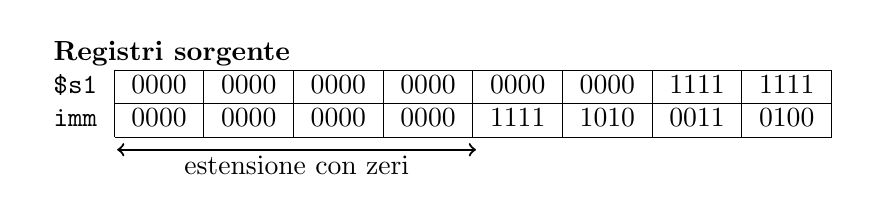
\begin{tikzpicture}
            \node(table) {
                \begin{tabular}{ c | c | c | c | c | c | c | c | c | }
                    \multicolumn{9}{ l }{\textbf{Registri sorgente}} \\
                    \cline{2-9}
                    \texttt{\$s1} & 0000 & 0000 & 0000 & 0000 & 0000 & 0000 & 1111 & 1111 \\
                    \cline{2-9}
                    \texttt{imm} & 0000 & 0000 & 0000 & 0000 & 1111 & 1010 & 0011 & 0100 \\
                    \cline{2-9}
                \end{tabular}
            };
    
            \draw [<->, thick]
                (-4.03,-.8) -- (.527,-.8);
    
            \node[text width=4.3cm, align=center] at (-1.75,-1) {estensione con zeri};
    
        \end{tikzpicture}
    \end{minipage}

    \vspace*{2mm}

    \begin{tabular}{ l p{1.7mm} c | c | c | c | c | c | c | c | c | }
        \textbf{Codice assembly} & & \multicolumn{9}{ l }{\textbf{Risultato}} \\
        \cline{4-11}
        \texttt{andi \$s2, \$s1, 0xFA34} & & \texttt{\$s2} & 0000 & 0000 & 0000 & 0000 & 0000 & 0000 & 0011 & 0100 \\
        \cline{4-11}
        \texttt{ori \$s3, \$s1, 0xFA34} & & \texttt{\$s3} & 0000 & 0000 & 0000 & 0000 & 1111 & 1010 & 1111 & 1111 \\
        \cline{4-11}
        \texttt{xori \$s4, \$s1, 0xFA34} & & \texttt{\$s4} & 0000 & 0000 & 0000 & 0000 & 1111 & 1010 & 1100 & 1011 \\
        \cline{4-11}
    \end{tabular}
\end{table}

\newpage

\subsection*{Esercizio}
L'istruzione \texttt{nori} non fa parte del set di istruzioni MIPS
perché la stessa funzionalità può essere implementata usando
delle istruzioni già esistenti. \\
Scrivere un breve comando assembly che abbia la seguente funzionalità:
\begin{center}
    \texttt{\$t0 = \$t1 NOR 0xF234}
\end{center}
\underline{\textbf{Nota}: usare meno istruzioni possibili.}
\\[.5cm]
\textbf{Soluzione} \\
\texttt{ORI \$t0, \$t1, 0xF234} \\
\texttt{NOR \$t0, \$t0, \$0}

\subsection{Istruzioni di shift}
Il campo che determina il numero di posizioni da shiftare è lo \texttt{shamt}.
\begin{table}[h!]
    \centering

    \setlength{\tabcolsep}{0pt}
    \begin{tabular}{ c c | c | c | c | c | c | c }
        \vspace*{-4.2mm} & \multicolumn{1}{ p{(\linewidth / 48) * 6} }{} & \multicolumn{1}{ p{(\linewidth / 48) * 5} }{} & \multicolumn{1}{ p{(\linewidth / 48) * 5} }{} & \multicolumn{1}{ p{(\linewidth / 48) * 5} }{} & \multicolumn{1}{ p{(\linewidth / 48) * 5} }{} & \multicolumn{1}{ p{(\linewidth / 48) * 6} }{} \\
        \cline{2-7}
        \multicolumn{1}{ c | }{} & \texttt{op} & \texttt{rs} & \texttt{rt} & \texttt{rd} & \textbf{\texttt{shamt}} & \texttt{funct} & \\
        \cline{2-7}
        \rule{0pt}{.8\normalbaselineskip} & \multicolumn{1}{ c }{6 bits} & \multicolumn{1}{ c }{5 bits} & \multicolumn{1}{ c }{5 bits} & \multicolumn{1}{ c }{5 bits} & \multicolumn{1}{ c }{5 bits} & \multicolumn{1}{ c }{6 bits} & \\
    \end{tabular}
\end{table}

\noindent
Le operazioni di shift possibili sono 3:
\begin{table}[h!]
    \centering

    \setlength{\tabcolsep}{24pt}
    \begin{tabular}{ c | c | c }
        \texttt{sll} & \texttt{srl} & \texttt{sra} \\
        \textit{''shift logico a sinistra"} & \textit{''shift logico a destra"} & \textit{''shift aritmetico a destra"} \\
    \end{tabular}
\end{table}

\noindent
Esempi:
\begin{itemize}
    \item \texttt{sll \$t0, \$t1, 5  \hspace*{0cm} \hspace*{0cm} \# \$t0 <= \$t1 << 5}
    \item \texttt{srl \$t0, \$t1, 5  \hspace*{0cm} \hspace*{0cm} \# \$t0 <= \$t1 >> 5}
    \item \texttt{sra \$t0, \$t1, 5  \hspace*{0cm} \hspace*{0cm} \# \$t0 <= \$t1 >>> 5}
\end{itemize}

\vspace*{5mm}

\noindent
\underline{\textbf{Nota bene}: queste istruzioni non sono di tipo I
nonostante utilizzino una costante (sono di tipo R).}

\subsubsection{Shift logico}
\vspace*{-4mm}
\begin{table}[h!]
    \begin{minipage}{.02\linewidth}
        \hspace*{0cm}
    \end{minipage}
    \begin{minipage}{.45\linewidth}
        \textbf{a sinistra} \\
        \textit{''va a spostare la \texttt{word} dal registro sorgente al registro
        destinazione caricando il registro di destinazione
        con bit a 0 nelle cifre \underline{meno significative}"}
        \underline{Con i numeri senza segno questo equivale ad una}
        \underline{moltiplicazione per una potenza di
        $2^{{<\text{numero di shift}>}}$.}

        \vspace*{3mm}

        \centering

        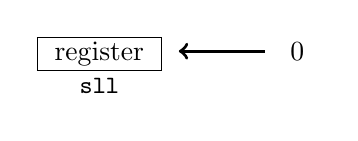
\begin{tikzpicture}
            \node(table) {
                \begin{tabular}{ c p{1cm} c }
                    \cline{1-1}
                    \multicolumn{1}{ | c |}{register} & & 0 \\
                    \cline{1-1}
                    \small \texttt{sll} \\
                \end{tabular}
            };
    
            \draw [<-, very thick]
                (0,.24) -- (1.1,.24);

        \end{tikzpicture}
    \end{minipage}
    \begin{minipage}{.08\linewidth}
        \hspace*{0cm}
    \end{minipage}
    \begin{minipage}{.45\linewidth}
        \textbf{a destra} \\
        \textit{''va a spostare la \texttt{word} dal registro sorgente al registro
        destinazione caricando il registro di destinazione
        con bit a 0 nelle cifre \underline{più significative}"} \\
        \underline{Con i numeri senza segno questo equivale ad una}
        \underline{divisione per una potenza di
        $2^{{<\text{numero di shift}>}}$.}

        \vspace*{3mm}

        \centering

        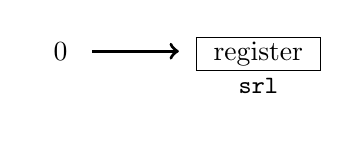
\begin{tikzpicture}
            \node(table) {
                \begin{tabular}{ c p{1cm} c }
                    \cline{3-3}
                    0 & & \multicolumn{1}{ | c |}{register} \\
                    \cline{3-3}
                    & & \small \texttt{srl} \\
                \end{tabular}
            };
    
            \draw [->, very thick]
                (-1.1,.24) -- (0,.24);

        \end{tikzpicture}
    \end{minipage}
\end{table}

\noindent
\textbf{Esempio} \\
Dato il numero \texttt{00 00 10 10}, con lo shift logico: \\
\hspace*{-2.2mm}
\begin{tabular}{ c l p{2mm} r c l }
    & • \hspace{-.5mm} a sinistra ottengo & & \texttt{00 10 10 00} \\
    & • \hspace{-.5mm} a destra ottengo & & \texttt{00 00 00 10} & & (i bit meno significativi vengono persi) \\
\end{tabular}

\subsubsection{Shift aritmetico}
Lo shift aritmetico mi permette di fare una divisione per numeri in
complemento a 2 (con segno).

\begin{table}[h!]
    \centering

    \hspace*{-6.48mm}
    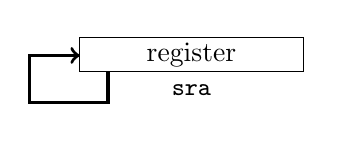
\begin{tikzpicture}
        \node(table) {
            \setlength{\tabcolsep}{24pt}
            \begin{tabular}{ c }
                \hline
                \multicolumn{1}{ | c | }{register} \\
                \hline
                \small \texttt{sra} \\
            \end{tabular}
        };

        \draw [->, very thick]
            (-1,0) |- (-2,-.4) -| (-2, .2) |- (-1.36, .2);
    
    \end{tikzpicture}
\end{table}

\noindent
\textbf{Esempio} \\
Dato il numero \texttt{1100} ($-$4), con lo shift aritmetico a destra
ottengo \texttt{1110} ($-$2 = \nicefrac{$-$4}{2}).

\newpage

\subsubsection{Shift variabile}
Esistono anche le varianti delle istruzioni precedenti,
con il numero di shift definito con una variabile \\
anziché con un valore immediato. \\
Piuttosto di andare a leggere una costante, vado a leggere
il valore di un registro. \\
Le operazioni possibili sono sempre 3:
\begin{table}[h!]
    \centering

    \setlength{\tabcolsep}{24pt}
    \begin{tabular}{ c | c | c }
        \texttt{sllv} & \texttt{srlv} & \texttt{srav} \\
        \makecell{\textit{''shift logico variabile} \\ \textit{a sinistra"}} & \makecell{\textit{''shift logico variabile} \\ \textit{a destra"}} & \makecell{\textit{''shift aritmetico variabile} \\ \textit{a destra"}} \\
    \end{tabular}
\end{table}

\noindent
Esempi:
\begin{itemize}
    \item \texttt{sllv \$t0, \$t1, \$t2 \hspace*{0cm} \hspace*{0cm} \# \$t0 <= \$t1 << \$t2}
    \item \texttt{srlv \$t0, \$t1, \$t2 \hspace*{0cm} \hspace*{0cm} \# \$t0 <= \$t1 >> \$t2}
    \item \texttt{srav \$t0, \$t1, \$t2 \hspace*{0cm} \hspace*{0cm} \# \$t0 <= \$t1 >>> \$t2}
\end{itemize}

\vspace*{5mm}

\noindent
\underline{\textbf{Nota bene}: si dice variabile in quanto all'interno
del codice posso variare il numero di bit per cui} \\
\underline{faccio lo shift.}

\subsection*{Esempio}
\texttt{sll \$t0, \$s1, 2} \\
\texttt{srl \$s2, \$s1, 2} \\
\texttt{sra \$s3, \$s1, 2} \\

\begin{table}[h!]
    \centering

    \caption*{\textbf{Valori dei campi}}
    \setlength{\tabcolsep}{0pt}
    \begin{tabular}{ c | c | c | c | c | c | c | c }
        \vspace*{-4.2mm} & \multicolumn{1}{ p{(\linewidth / 48) * 6} }{} & \multicolumn{1}{ p{(\linewidth / 48) * 5} }{} & \multicolumn{1}{ p{(\linewidth / 48) * 5} }{} & \multicolumn{1}{ p{(\linewidth / 48) * 5} }{} & \multicolumn{1}{ p{(\linewidth / 48) * 5} }{} & \multicolumn{1}{ p{(\linewidth / 48) * 6} }{} \\
        \\[-9mm]
        \multicolumn{1}{ c }{\multirow{2}{*}{}} &
        \multicolumn{1}{ c }{\multirow{2}{*}{op}} &
        \multicolumn{1}{ c }{\multirow{2}{*}{rs}} &
        \multicolumn{1}{ c }{\multirow{2}{*}{rt}} &
        \multicolumn{1}{ c }{\multirow{2}{*}{rd}} &
        \multicolumn{1}{ c }{\multirow{2}{*}{shamt}} &
        \multicolumn{1}{ c }{\multirow{2}{*}{funct}} &
        \\[-4.4mm]
        & & & & & & \\[2.4mm]
        \cline{2-7}
        \multicolumn{1}{ c | }{} & 0 & 0 & 17 & 8 & 2 & 0 & \\
        \cline{2-7}
        \multicolumn{1}{ c | }{} & 0 & 0 & 17 & 18 & 2 & 2 & \\
        \cline{2-7}
        \multicolumn{1}{ c | }{} & 0 & 0 & 17 & 19 & 2 & 3 & \\
        \cline{2-7}
        \multicolumn{1}{ c }{\rule{0pt}{.8\normalbaselineskip}} & \multicolumn{1}{ c }{6 bits} & \multicolumn{1}{ c }{5 bits} & \multicolumn{1}{ c }{5 bits} & \multicolumn{1}{ c }{5 bits} & \multicolumn{1}{ c }{5 bits} & \multicolumn{1}{ c }{6 bits} & \\
    \end{tabular}
\end{table}
\vspace*{-5mm}
\begin{table}[h!]
    \centering
    \huge $\Downarrow$
\end{table}
\vspace*{-3mm}
\begin{table}[h!]
    \centering

    \begin{minipage}{.1\linewidth}
        \hspace*{0cm}
    \end{minipage}
    \begin{minipage}{.75\linewidth}
        \centering

        \caption*{\textbf{Codice macchina}}
        \setlength{\tabcolsep}{0pt}
        \begin{tabular}{ c | c | c | c | c | c | c | c }
            \vspace*{-4.2mm} & \multicolumn{1}{ p{(((\linewidth / 48) * 4) / 3) * 6} }{} & \multicolumn{1}{ p{(((\linewidth / 48) * 4) / 3) * 5} }{} & \multicolumn{1}{ p{(((\linewidth / 48) * 4) / 3) * 5} }{} & \multicolumn{1}{ p{(((\linewidth / 48) * 4) / 3) * 5} }{} & \multicolumn{1}{ p{(((\linewidth / 48) * 4) / 3) * 5} }{} & \multicolumn{1}{ p{(((\linewidth / 48) * 4) / 3) * 6} }{} \\
            \\[-9mm]
            \multicolumn{1}{ c }{\multirow{2}{*}{}} &
            \multicolumn{1}{ c }{\multirow{2}{*}{op}} &
            \multicolumn{1}{ c }{\multirow{2}{*}{rs}} &
            \multicolumn{1}{ c }{\multirow{2}{*}{rt}} &
            \multicolumn{1}{ c }{\multirow{2}{*}{rd}} &
            \multicolumn{1}{ c }{\multirow{2}{*}{shamt}} &
            \multicolumn{1}{ c }{\multirow{2}{*}{funct}} &
            \\[-4.4mm]
            & & & & & & \\[2.4mm]
            \cline{2-7}
            \multicolumn{1}{ c | }{} & 000000 & 00000 & 10001 & 01000 & 00010 & 000000 \\
            \cline{2-7}
            \multicolumn{1}{ c | }{} & 000000 & 00000 & 10001 & 10010 & 00010 & 000010 \\
            \cline{2-7}
            \multicolumn{1}{ c | }{} & 000000 & 00000 & 10001 & 10011 & 00010 & 000011 \\
            \cline{2-7}
            \multicolumn{1}{ c }{\rule{0pt}{.8\normalbaselineskip}} & \multicolumn{1}{ c }{6 bits} & \multicolumn{1}{ c }{5 bits} & \multicolumn{1}{ c }{5 bits} & \multicolumn{1}{ c }{5 bits} & \multicolumn{1}{ c }{5 bits} & \multicolumn{1}{ c }{6 bits} \\
        \end{tabular}
    \end{minipage}
    \begin{minipage}{.1\linewidth}
        \vspace*{5mm}

        \texttt{\hspace*{-9.5mm} (0x00114080)}
        \texttt{\hspace*{-9.5mm} (0x00119082)}
        \texttt{\hspace*{-9.5mm} (0x00119883)}
    \end{minipage}
\end{table}

\newpage

\end{document}